\documentclass[]{article}

\usepackage[english]{babel}
\usepackage[utf8]{inputenc}
\usepackage{amsmath}
\usepackage{graphicx}
\begin{document}

\title{Electronique II}
\author{Dylan Bourgeois}
\date{MT BA4}
\maketitle

\section{Introduction}
Cours d'électronique II, donné par Mme Lacour.

\section{Polarisation et Jonction PN}
\subsection{Physique du semi-conducteur}

\begin{itemize}
\item \textbf{Conducteurs :} $\rho < 10^{-5} [\Omega . cm]$ 
\item \textbf{Diélectriques :} $\rho > 10^{8} [\Omega . cm]$ 
\item \textbf{Semi-conducteurs :} $10^{-5} < \rho < 10^{8} [\Omega . cm]$  Conduction électrique par $e^-$ et trous.
 En apportant de l'énergie on fait passer les $e^-$ de la bande de valence (BV) à la bande de conduction (BC).

Densité de charges : $$ n_i = 5,2.10^{-15}T^{\frac{3}{2}} \exp{(-\frac{E_g}{2kT})} \quad [e^-.cm^{-3}] $$
Dans un semi-conducteur intrinsèque : $$ n = p = n_i \quad \quad \quad np = n_i^2 $$

\textbf{Conductivité électrique} dans un semi-conducteur : $\sigma = \mu_nne + \mu_ppe $

\textbf{Mobilité $\mu$} : $\quad v =\mu E\quad\quad [m.s^{-1}]=[m^2.V^{-1}.s^{-1}].[V.m^{-1}]$

\textbf{Courant :} $I = nqvtw=nq\mu Etw \;$ avec tw = surface et la densité de courant est $ j=\frac{I}{tw}=ne\mu E $

\textbf{Loi d'Ohm :} $ E = \frac{V}{l} \Rightarrow I= ne\mu \frac{tw}{l}.V $ avec la conductance $G=ne\mu \frac{tw}{l}$. 

La résistivité est donnée par $\rho=\frac{1}{ne\mu}$

\subsection{Dopage}
\subsubsection{Dopage N}
Inclusion d'impuretés qui donnent des $e^-$ dans la BC.
$$ n=N_D \Rightarrow p = \frac{n_i^2}{N_D} \quad avec \quad 10^{15} < N_D < 10^{20}\; cm^{-3}$$
\subsubsection{Dopage P}
Inclusion d'impuretés qui donnent des trous dans la BC.
$$  n=N_A \Rightarrow p = \frac{n_i^2}{N_A} $$

\end{itemize}

\subsection{Jonctions PN}
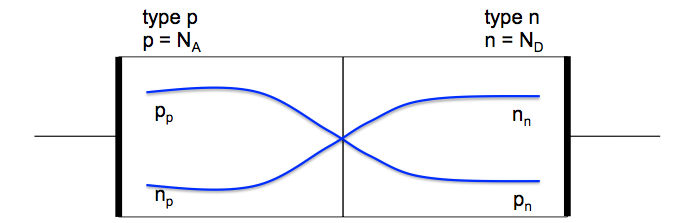
\includegraphics[scale=0.4]{pn}

\subsection{Zone de dépletion}
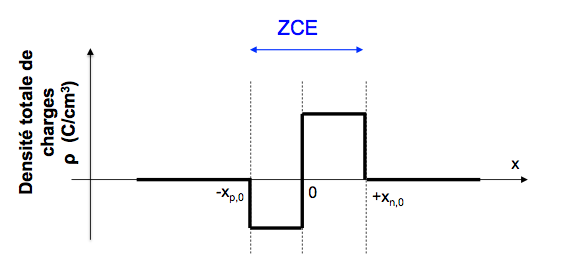
\includegraphics[scale=0.35]{dcharges}
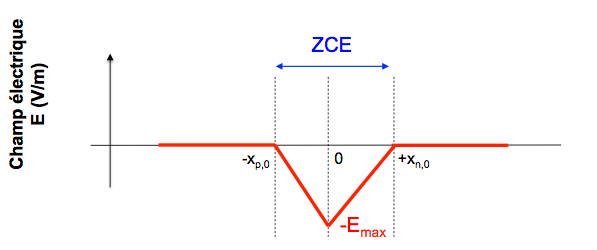
\includegraphics[scale=0.35]{delec}
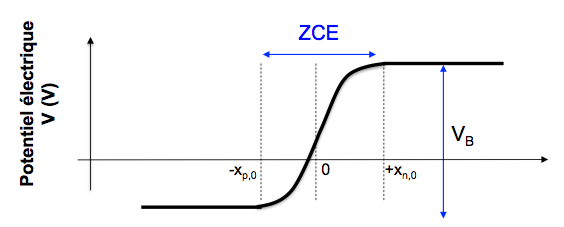
\includegraphics[scale=0.4]{pelec}
$ V_B = \frac{kT}{q}\ln{(\frac{N_AN_D}{n_i^2})}$

\subsection{Capacité de déplétion}
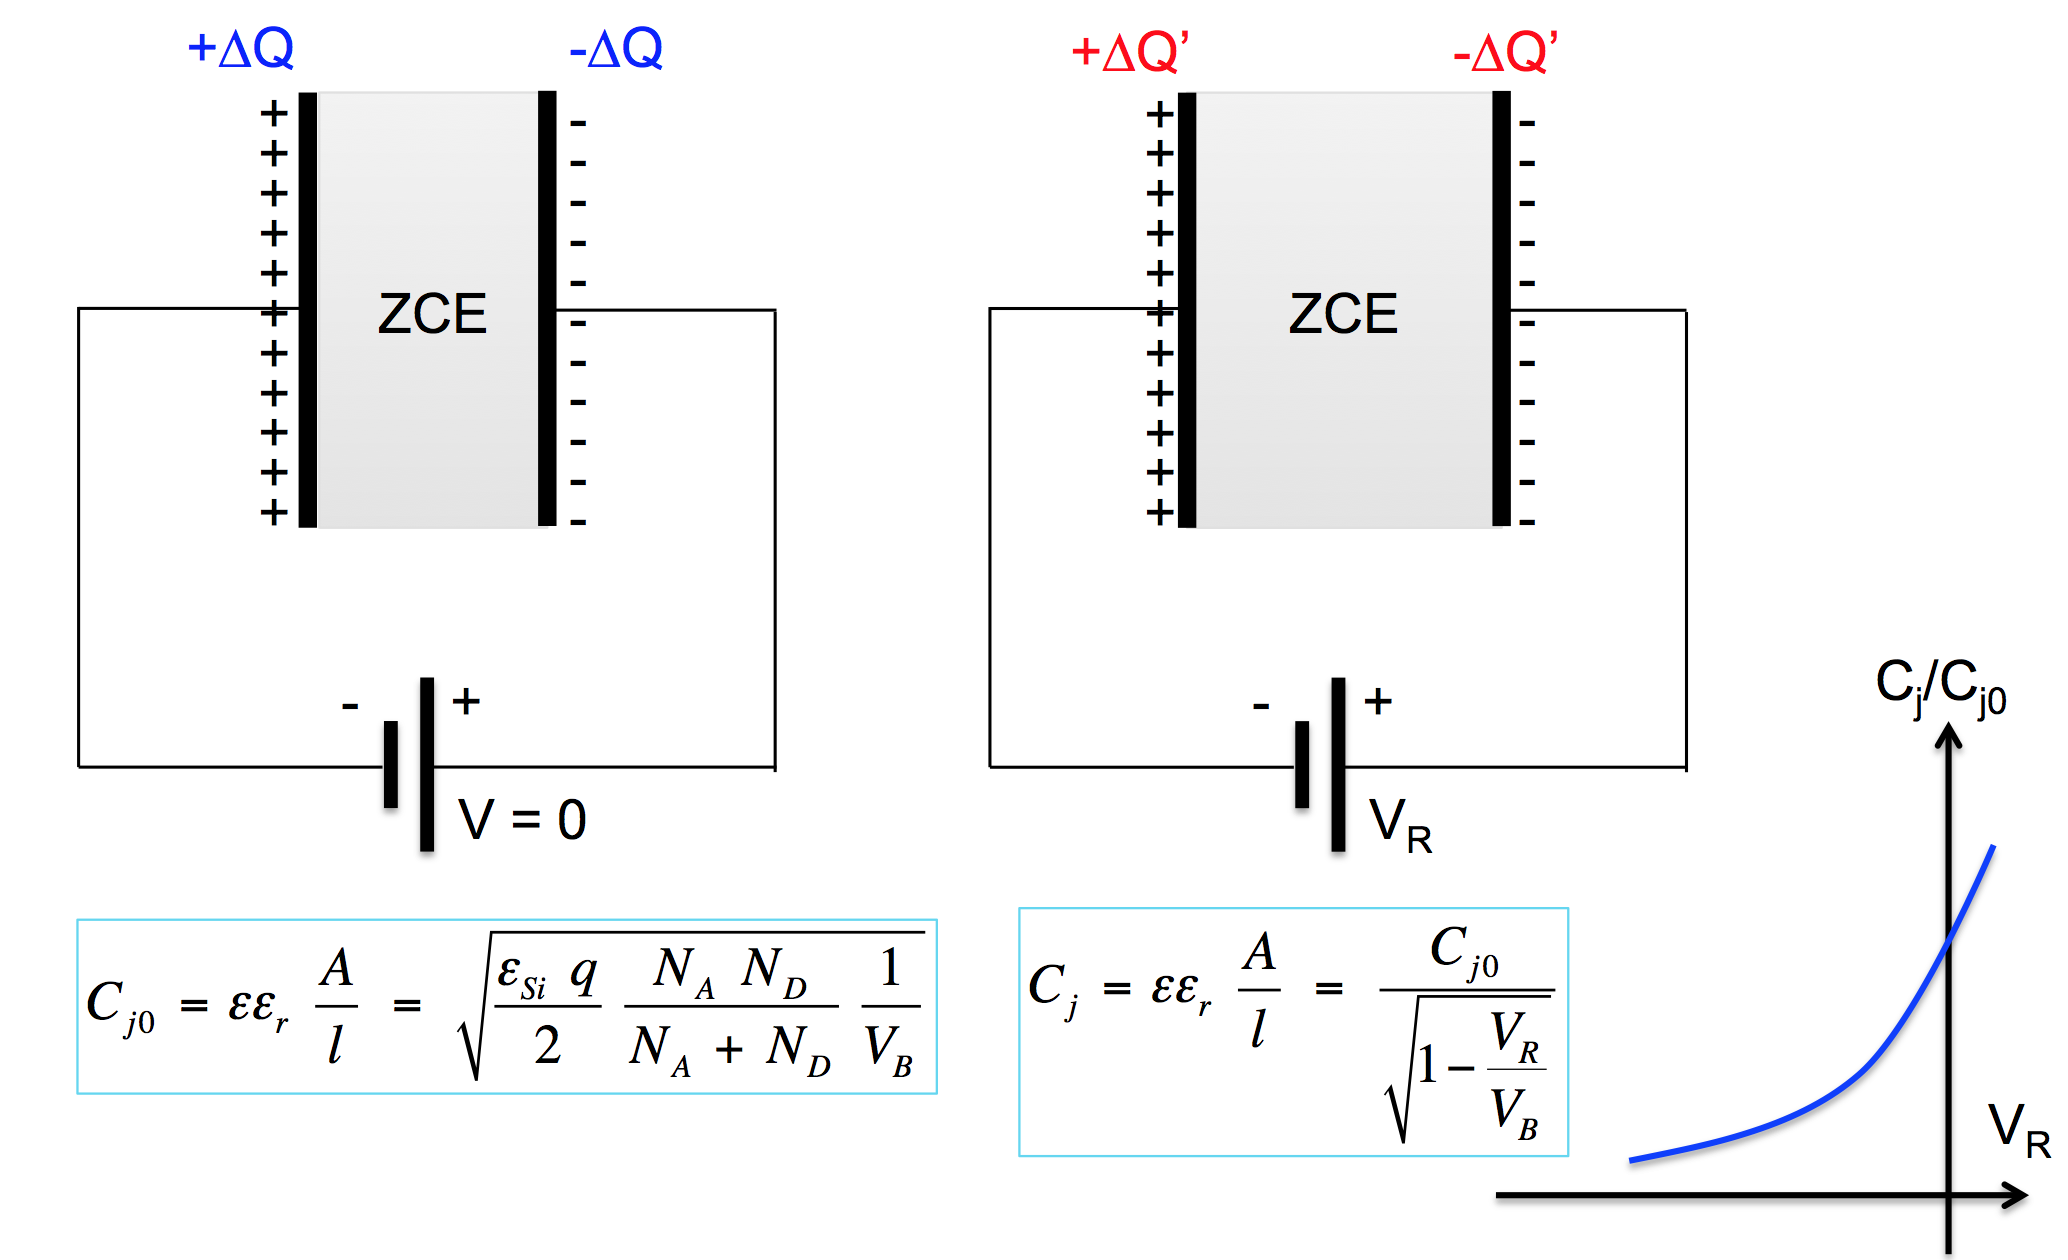
\includegraphics[scale=0.3]{capa}

\subsection{Caractéristique $I(V)$}
$ I_D = I_S \exp{(\frac{V_D}{V_T}-1)} $

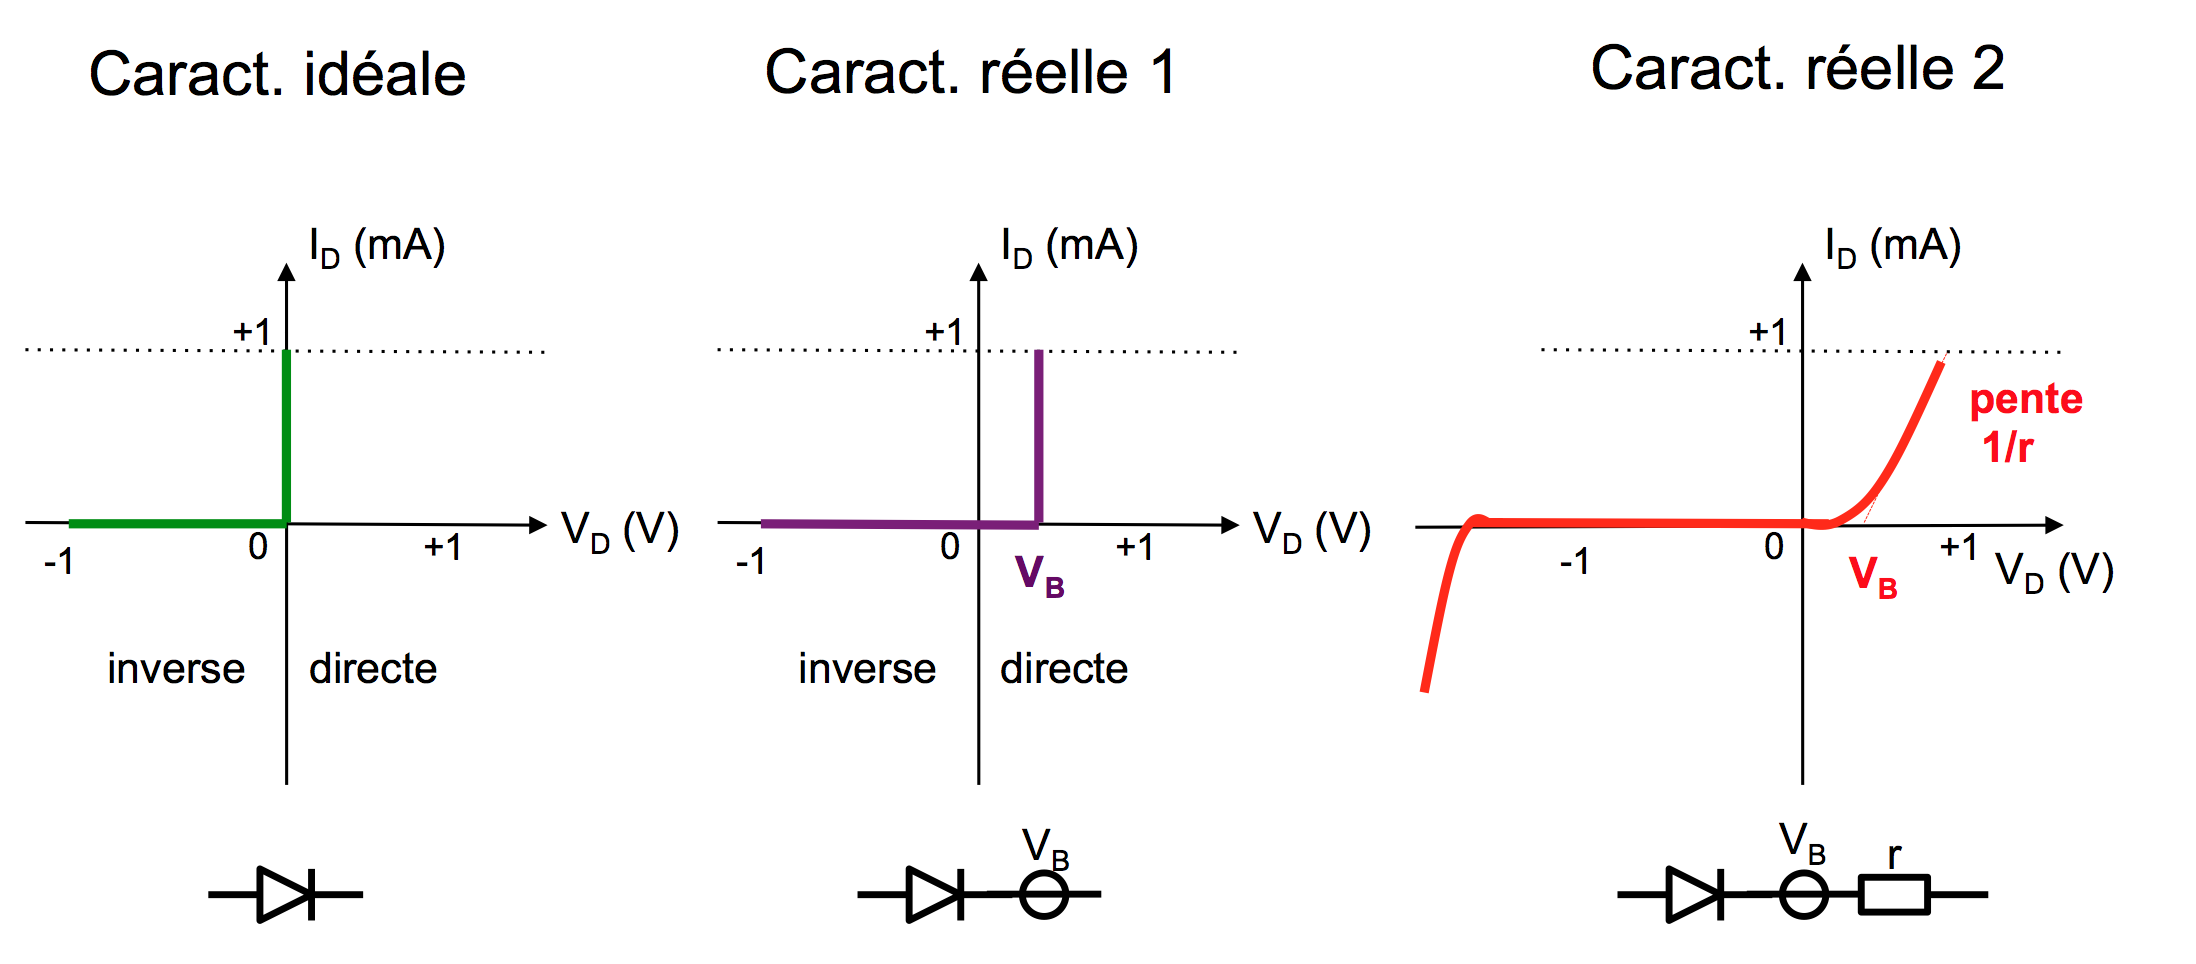
\includegraphics[scale=0.3]{car}

\subsection{Courant de diode}
\subsubsection{$V_D < 0$}
$$ I_D \sim - I_S = A\frac{kT}{q}(\mu_p\frac{n_i^2}{N_DL_p}+\mu_n\frac{n_i^2}{N_AL_n}) $$

\subsubsection{$V_D > 0$}

$$ ideal : \; I_D = I_S(\exp {\frac{qV_D}{kT}} -1) \quad reel : \;  I_D = I_S(\exp {\frac{qV_D}{nkT}} -1) $$

\subsection{Diode Zener}
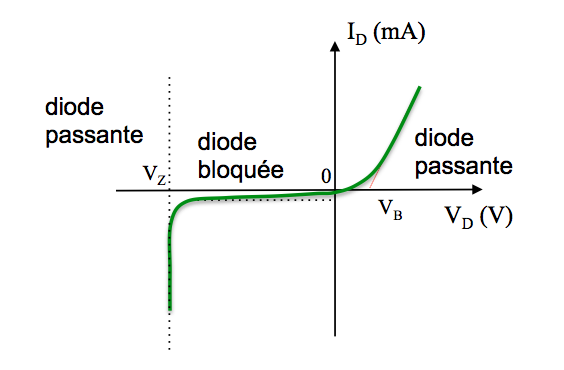
\includegraphics[scale=0.8]{zener_IV.png} 
\subsection{A retenir}

La polarisation d'une jonction PN modifie la distribution des charges à la surface:

-  \textbf{Polarisation directe} : les porteurs minoritaires sont injectés dans les "zones neutres"

- \textbf{Polarisation inverse} : les porteurs minoritaires sont arrachés dans les "zones neutres"

Caractéristique $I(V)$ de la diode PN : $$ I_D \approx I_s \exp{(\frac{qV_D}{nkT})} $$

Paramètres essentiels : $V_B , - I_s, r_d$

\section{Le transistor bipolaire}
\subsection{Structure du transistor}
\subsubsection{Le transistor}
Polarité indiquée par la flèche ($=$ direction du courant $I_E$)
Comporte trois électrodes :

- \textbf{Base} : électrode de commande.

- \textbf{Collecteur} : Relié au $\oplus$ de l'alimentation.

- \textbf{Emetteur} : draine les courants de base et de collecteur.

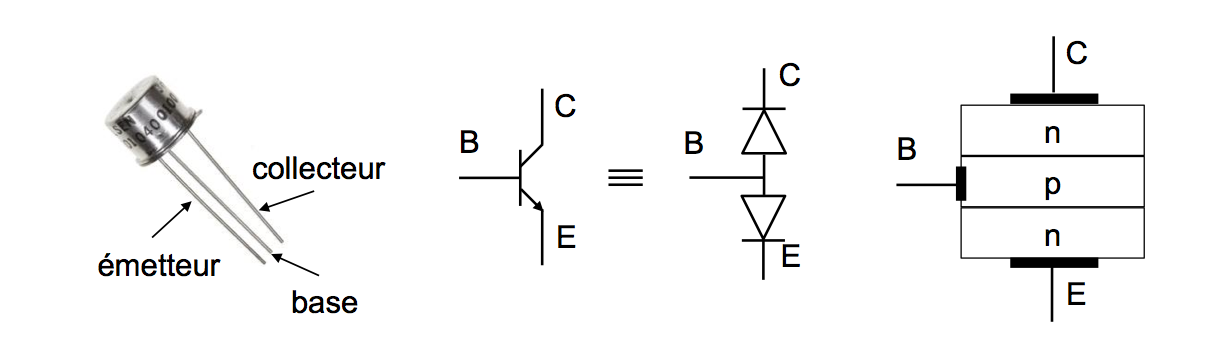
\includegraphics[scale=0.6]{transistor.png} 

\subsubsection{Transistor NPN}

\begin{itemize}
\item \textbf{Etats de fonctionnement} :\quad \quad
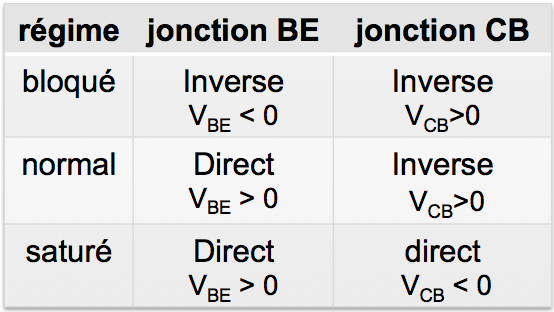
\includegraphics[scale=0.6]{npn_etats.png} 

\item \textbf{Fonctionnement normal} :
La "diode" BE est polarisée en mode direct, donc $V_{BE} > 0$. Les courants de diffusion sont des porteurs majoritaires : Trous de $B\rightarrow E$, $e^-$ de $E\rightarrow B$.
La "diode" BC est ploarisée en mode inverse, donc $V_{BC} <  0$.  Les courants de diffusion sont des porteurs minoritaires :  $e^-$ de $B\rightarrow C$.
Au final, une large portion d'$e^-$ se déplacent de $E\rightarrow C$, et un faible courant de trous se déplacent de $B \rightarrow E$.
\end{itemize}

\subsubsection{Les courants $I_B,I_E,I_C$}

Courant de collecteur (\textbf{NB} : ne dépend que de $V_{BE}$) : 
$$I_C = I_S \exp{(\frac{V_{BE}}{U_T}-1)}$$ 

Courant de base (avec $\beta$ le gain en courant, $50 < \beta < 200$) : 
$$ I_B = \frac{I_C}{\beta} $$

Courant d'émetteur : $$ I_E =  ( \frac{1}{\beta} + 1 ) I_S \exp{(\frac{V_{BE}}{U_T}-1)}$$

\subsubsection{Autres modes de fonctionnement}
\begin{itemize}
\item \textbf{Bloqué :}

Les deux jonctions BE et BC sont en mode inverse
Aucun courant ne circule
Le collecteur est isolé de l'émetteur (circuit ouvert) ($V_{CE} \rightarrow V_{CC}$)
$$ i_B = i_C = i_E = 0 $$
\item \textbf{Saturé :}

Le deux jonctions BE et BC sont en mode direct : $V_{BE} \sim 0.7V$ et $ V_{BC} \sim 0.7V$.
Diminution de $V_{CE} \rightarrow V_{CE,sat} \sim 0.2-0.3V$
Augmentation du courant de base $i_B$ jusqu'à $i_{B,sat} > \frac{i_{C,sat}}{\beta}$.
\end{itemize}

\subsubsection{A retenir}
En mode normal, les courants sont proportionnels entre-eux et au facteur $\exp{(\frac{V_{BE}}{V_T})}$. De plus $V_{BE}$ controle $I_C$ (effet transistor). Ce dernier est indépendant de $V_{BC}$ (isolation), mais est controlé via $I_B$.

\subsection{Caractéristiques I(V)}
\subsubsection{$I_C = f(V_{BE})$}
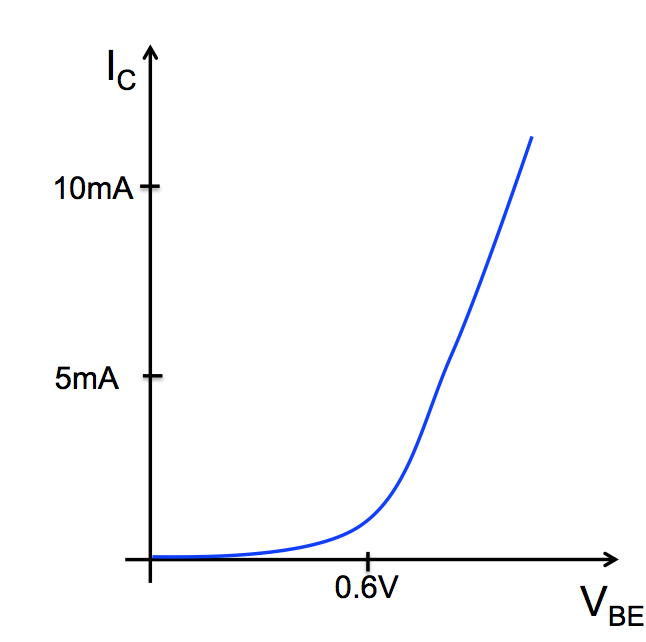
\includegraphics[scale=0.4]{Ic_Vbe.png}
\subsubsection{$I_C = f(I_B)$}
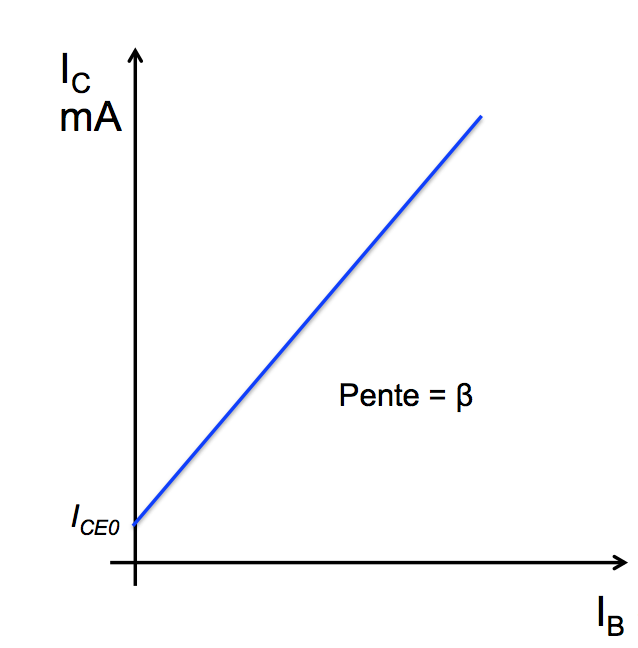
\includegraphics[scale=0.4]{Ic_Ib.png} 

Générateur de courant commandé par un courant. $I_{CE0}$ est le courant de fuite.
$$ 5< \beta < 80 : transistors\,de\,puissance \quad 100 < \beta < 500 : transistors\,de\,signal $$
\subsubsection{$I_C = f(V_{CE})$}
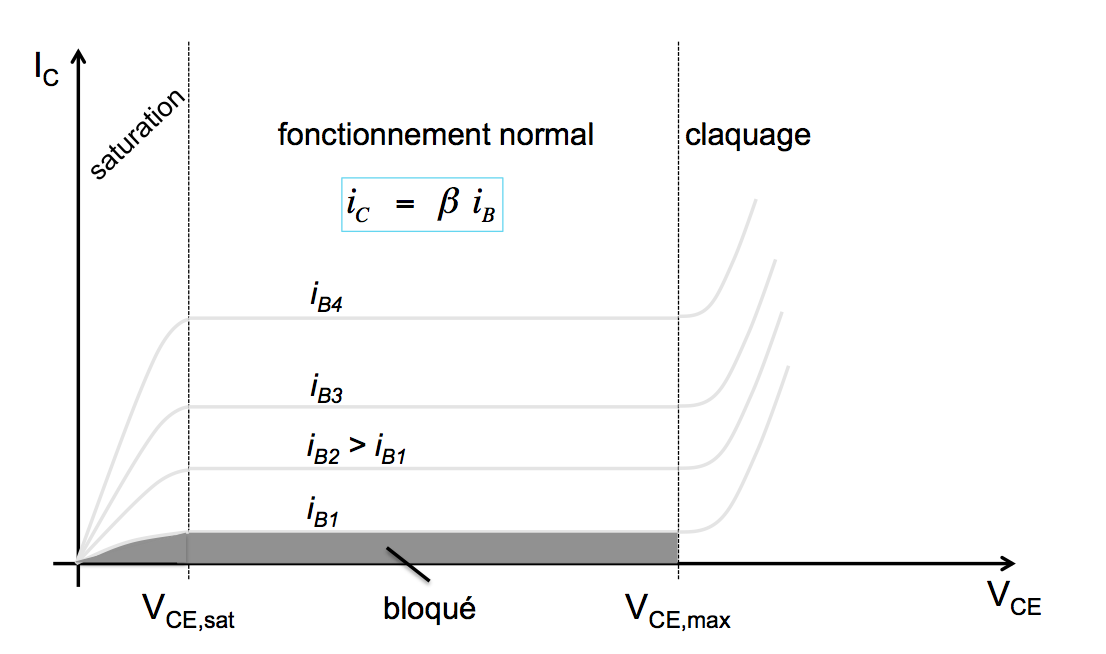
\includegraphics[scale=0.4]{Ic_Vce.png}

\subsubsection {Modèle grands signaux}
\begin{itemize}
\item \textbf{Blocage}$ V_{BE} < U_j ,\; I_C = 0A$
\item \textbf{Normal} 
\begin{itemize}
\item $V_{BE} = U_j , \; V_{BC} < U_j \;donc\; V_{CE}=V_{CB} + V_{BE} > 0 $

\item $I_C = \beta I_B $

\item $ I_E = (1+\beta)I_B \sim I_C $
\end{itemize}

\item \textbf{Saturation} 
\begin{itemize}
\item $ V_{BE} = V_{BC} = U_j \; donc\; V_{CE} = V_{CE,sat} \sim 0V$
\item $ I_B = I_{B,sat} > \frac{I_{C,sat}}{\beta} $ 
\end{itemize}
\end{itemize}

\subsubsection{Schémas équivalents}
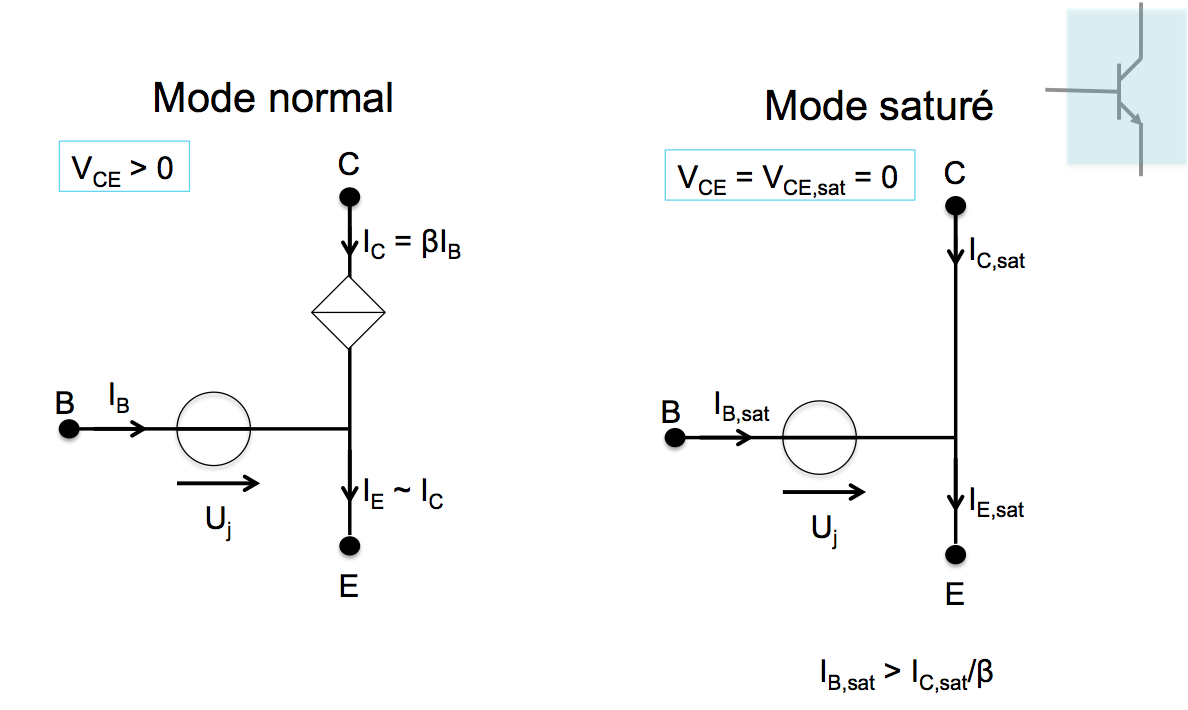
\includegraphics[scale=0.5]{schema_eq}
\subsubsection{Montage inverseur}
$V_X = V_{CC} - R_Ci_C$
\begin{itemize}
\item $V_1 \le U_j$ : Le transistor est bloqué et $V_X = V_{CC}$
\item $V_1 > U_j$ : Le transistor est passant et $V_X = V_{CC} - \beta R_Ci_B$
\item Si le transistor est saturé : $V_X = V_{CE,sat} \approx 0V$
\end{itemize}

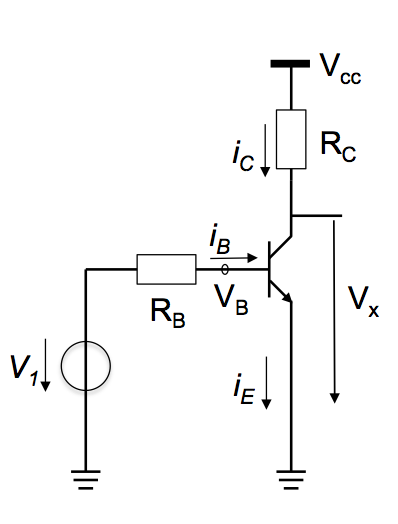
\includegraphics[scale=0.5]{inverseur}

\subsubsection{Transconductance}

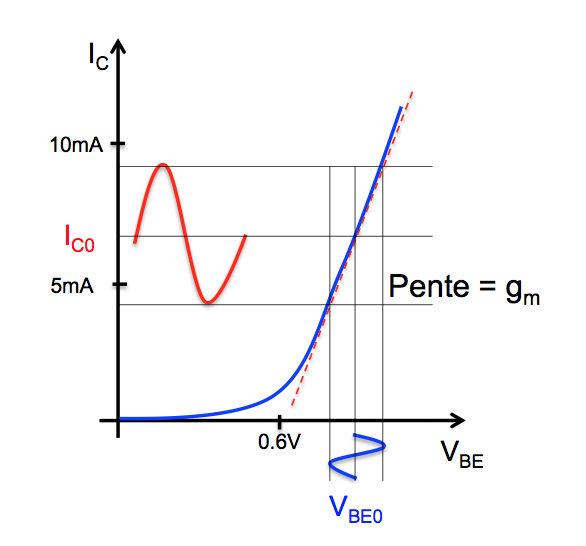
\includegraphics[scale=0.5]{transconductance.png}

$I_C = I_S(\exp{(\frac{V_{BE}}{U_T}-1)})$

$g_m = \frac{dI_C}{dV_{BE}}$

\subsection{Modèle petits signaux ($v \le 10 mV$)}
\subsubsection{Notations}
Composantes statiques et dynamiques :
\begin{itemize}
\item $ v_{BE}(t) = V_{BE,0} + v_{BE}(t) $
\item $ i_B(t) = I_{B,0} + i_B(t)$
\item $ v_{CE}(t) =  V_{CE,0} + v_{CE}(t) $
\item $ i_C(t) = I_{C,0} + i_C(t) $ 
\end{itemize}

\subsubsection{Transconductance}
$ g_m = \frac{i_c}{v_{BE}} = \frac{\partial I_C}{\partial V_{BE}}\mid_{V_{BE,0}\;,\;I_{C,0}} \Rightarrow g_m = \frac{I_{C,0}}{U_T}$

\subsubsection{Résistance d'entrée ($r_\pi$)}
$i_B = g_{be}v_{BE} \Rightarrow g_{be} = \frac{g_m}{\beta} = \frac{I_{C,0}}{\beta U_T} \quad \textbf{NB:} \; g_m >> g_{be}$

\subsubsection{Tension d'Early ($V_A$)}
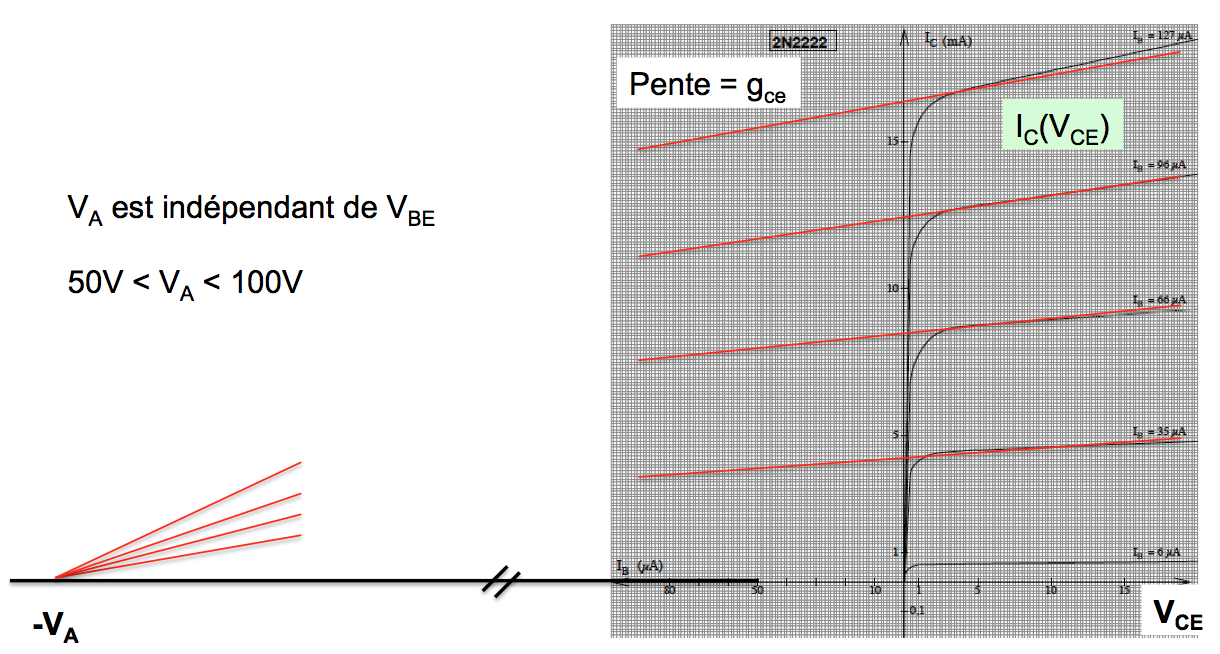
\includegraphics[scale=0.3]{early}

\subsubsection{Résistance de sortie ($r_0$)}
$i_c = g_{ce}v_{CE} \Rightarrow  \frac{i_c}{v_{CE}} = \frac{\partial I_C}{\partial V_{CE}}\mid_{V_{BE,0}\;,\;I_{C,0}} \Rightarrow g_{ce} = \frac{I_{C,0}}{V_A} \quad \textbf{NB:} \; g_m >> g_{be} >> g_{ce}$
\subsubsection{A retenir}
\begin{itemize}
\item \textbf{NPN}

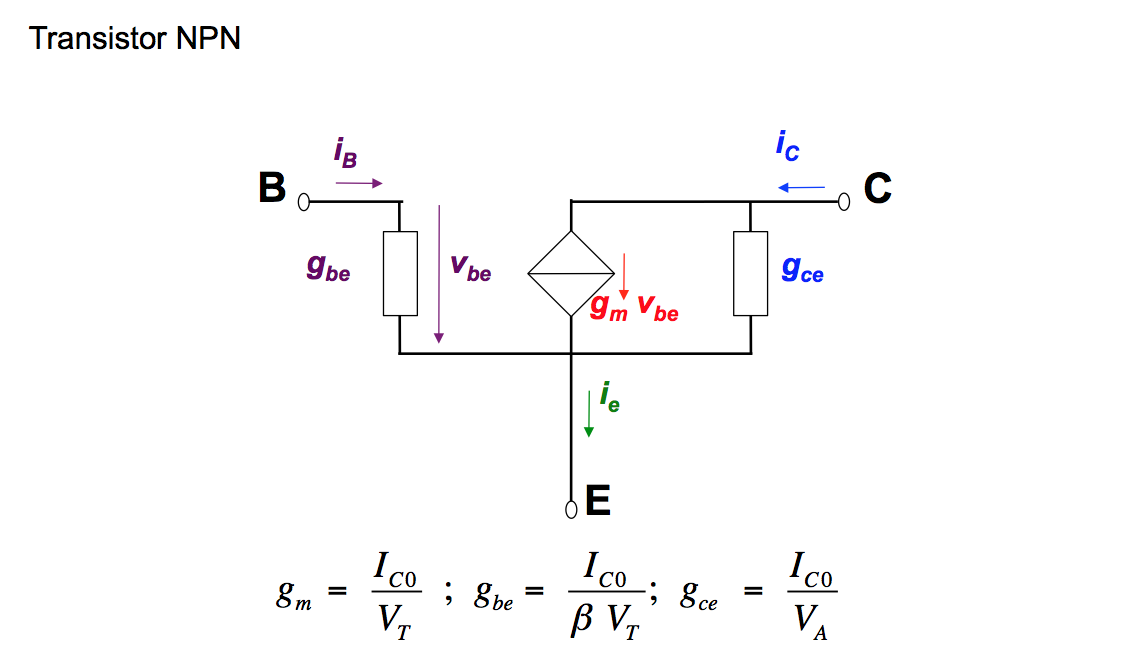
\includegraphics[scale=0.5]{aretenir_npn}

\item \textbf{PNP}

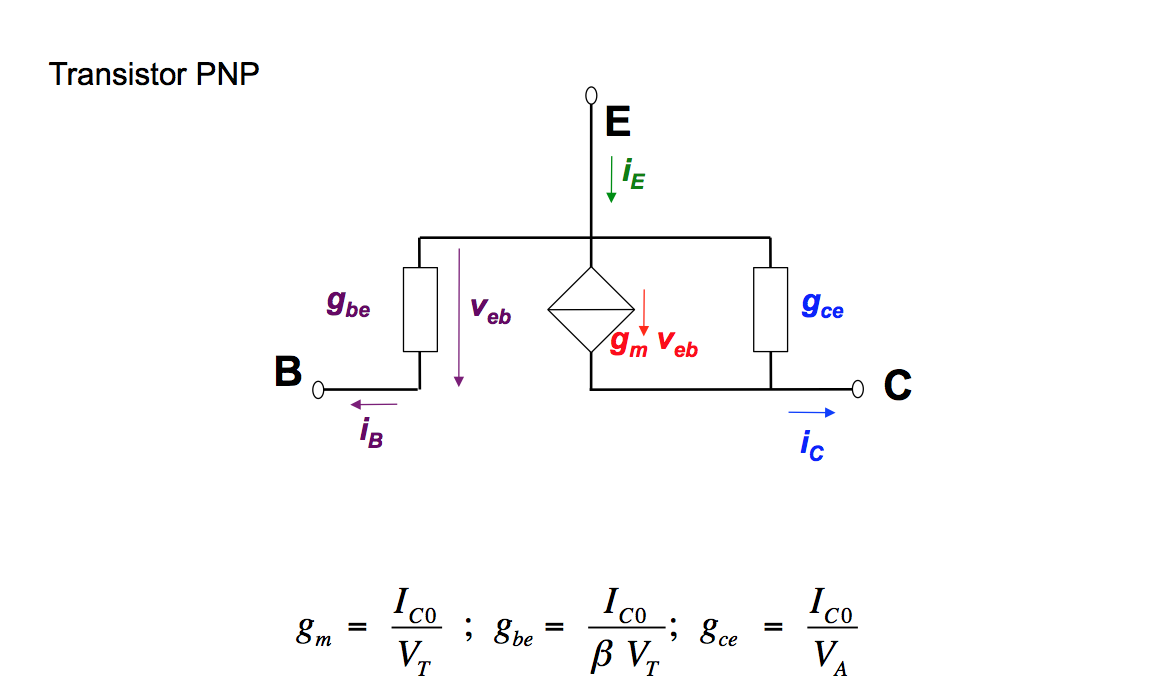
\includegraphics[scale=0.5]{aretenir_pnp}
\end{itemize}

\section{Modèle petits signaux}
\subsection{Quadripôle}
Le transistor peut-être vu comme un quadripôle si l'un des terminaux est mis en commun entre l'entrée et la sortie.

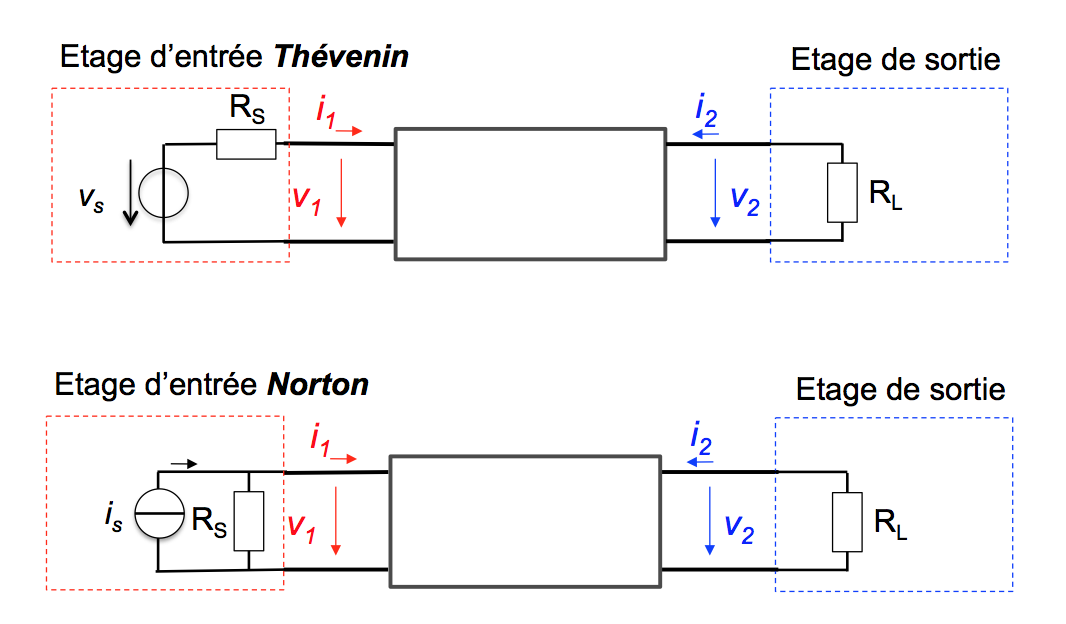
\includegraphics[scale=0.6]{quad}
\subsubsection{Résistance d'entrée}
$ R_{in} = \frac{v_1}{i_1}\mid_{R_L} $
\subsubsection{Impédance de sortie}
$ R_{out} = \frac{v_2}{i_2}\mid_{v_s=0} $
\subsubsection{Fonction de transfert}
Gains en tension :

\begin{itemize}
\item \textbf{Gain en tension à vide :} $A_{v,0} = \frac{v_2}{v_1}\mid_{R_L}\rightarrow\infty$
\item \textbf{Gain en tension avec une charge $R_L$ :} $ A_v =  \frac{v_2}{v_1}\mid_{R_L} = A_{v,0}\frac{R_L}{R_L + R_{out}}$
\end{itemize}
Gains en courant :
\begin{itemize}
\item \textbf{Gain en courant en court-circuit :} $A_{i,0} = \frac{i_2}{i_1}\mid_{R_L=0}$
\item \textbf{Gain en courant avec une charge $R_L$ :} $ A_i =  \frac{i_2}{i_1}\mid_{R_L} = A_{i,0}\frac{R_out}{R_L + R_{out}}$
\end{itemize}
Gains transconductance :
\begin{itemize}
\item \textbf{$G_{m,0}$ vide :} $G_{m,0} = \frac{i_2}{v_1}\mid_{R_L=0}$
\item \textbf{$G_{m}$ avec une charge $R_L$ :} $ G_m =  \frac{i_2}{i_1}\mid_{R_L} = G_{m,0}\frac{R_{out}}{R_L + R_{out}}$
\end{itemize}
Gains transrésistance :
\begin{itemize}
\item \textbf{$R_{m,0}$ à vide :} $R_{m,0} = \frac{i_2}{v_1}\mid_{R_L=0}$
\item \textbf{$R_{m}$ avec une charge  $R_L$:} $ R_m =  \frac{i_2}{i_1}\mid_{R_L} = R_{m,0}\frac{R_L}{R_L + R_{out}}$
\end{itemize}

\subsubsection{A retenir}
 \begin{itemize}
\item \textbf{A vide :} $A_{v,0} = - G_{m,0}R_{out}$
\item \textbf{Avec une charge  $R_L$:} $A_{v} = - G_{m}R_{L}$
\end{itemize}

\subsection{Applications au transistor bipolaire}
\subsubsection{Emetteur commun}
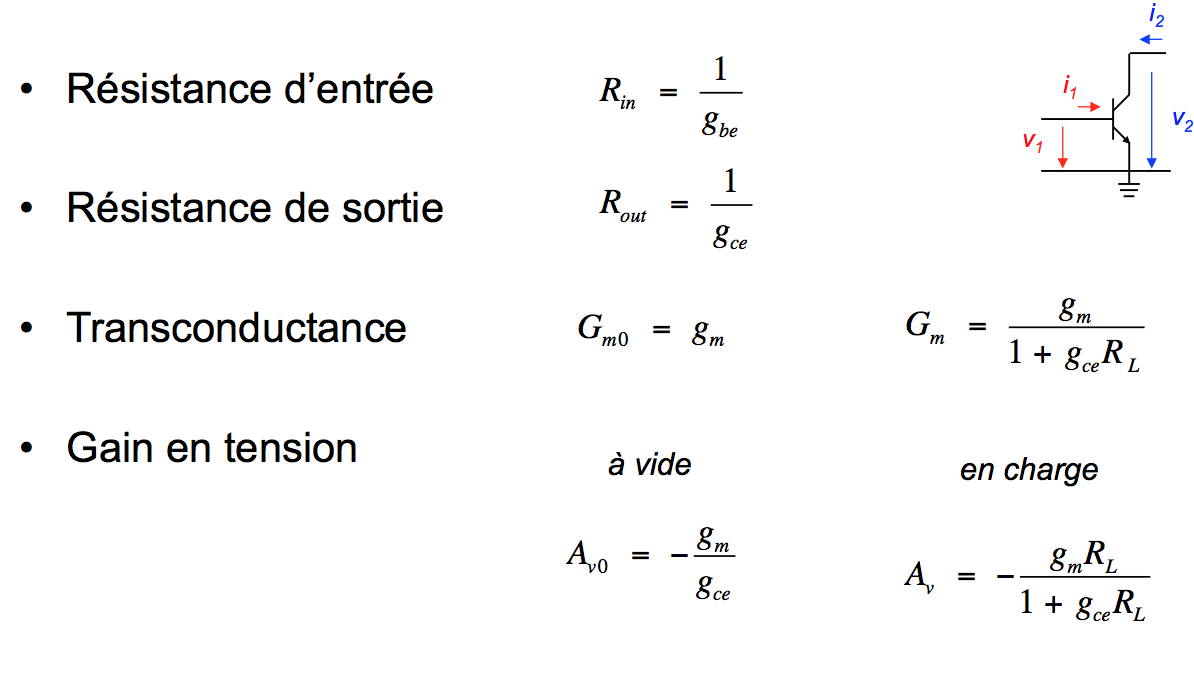
\includegraphics[scale=0.5]{emetteur}
\subsubsection{Base commune}
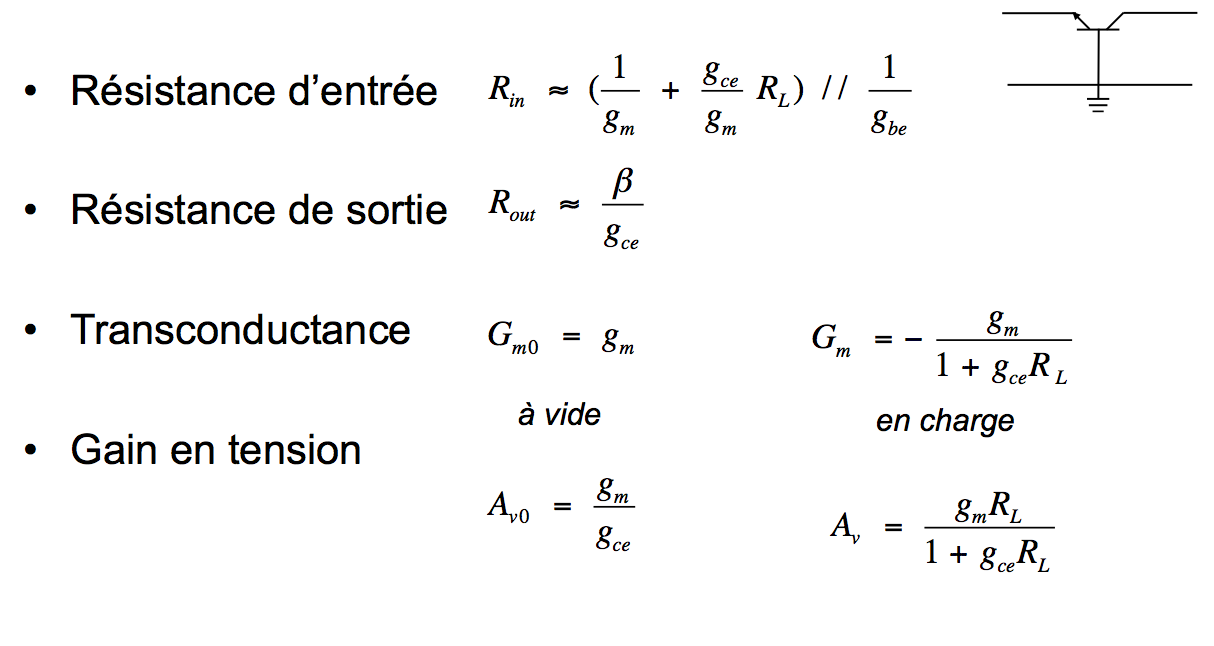
\includegraphics[scale=0.5]{base}
\subsubsection{Collecteur commun}
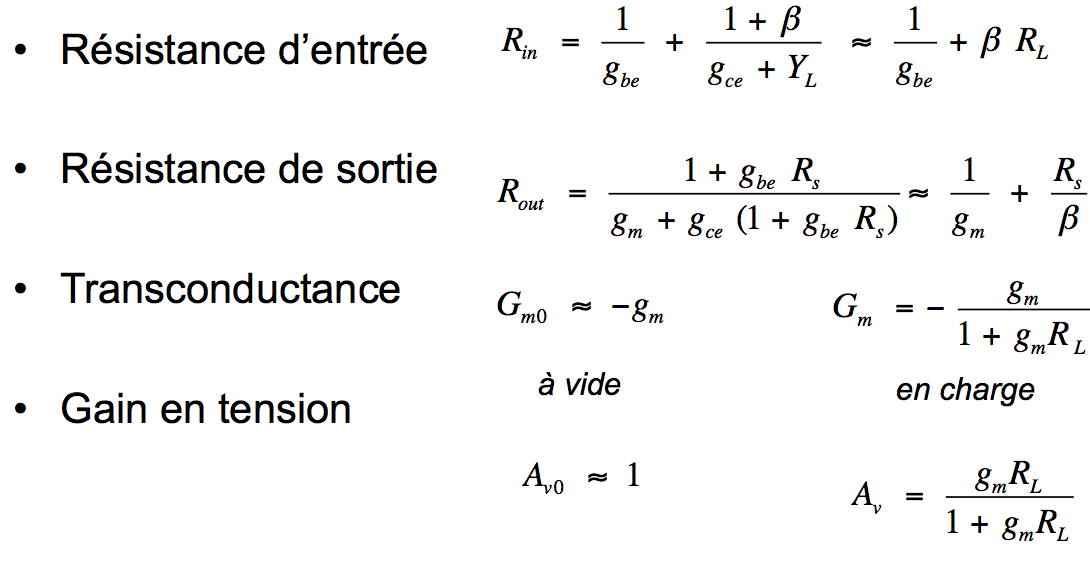
\includegraphics[scale=0.5]{coll}
\subsubsection{Comparaison}
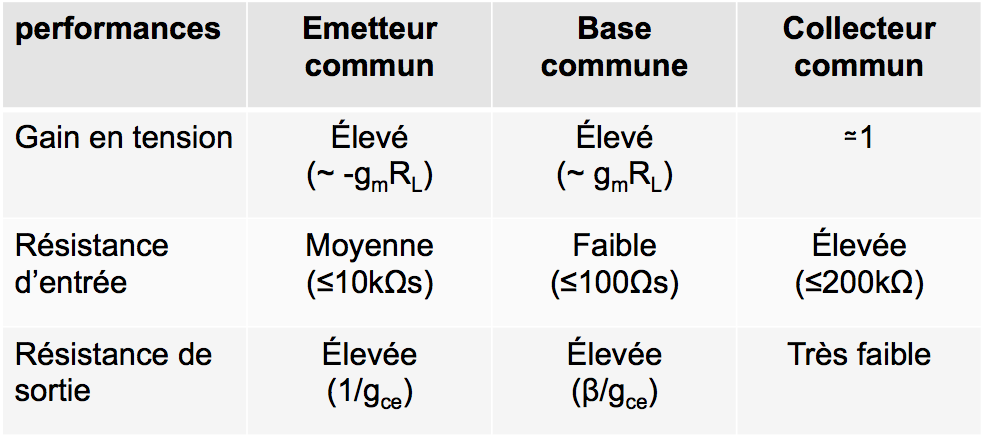
\includegraphics[scale=0.5]{comp}

\section{Polarisation}
\subsection{Rappel Condensateurs}
$ Z(jw) = \frac{1}{j\omega C} = \frac{1}{2\pi f C} $
Alors :
\begin{itemize}
\item \textbf{$f\rightarrow 0$  (i.e DC) :} condensateur $\sim$ circuit ouvert.
\item \textbf{$f\rightarrow \infty$ (i.e petits signaux) :} condensateur $\sim$ court-circuit.
\end{itemize}

\subsubsection{Condensateurs de couplage}
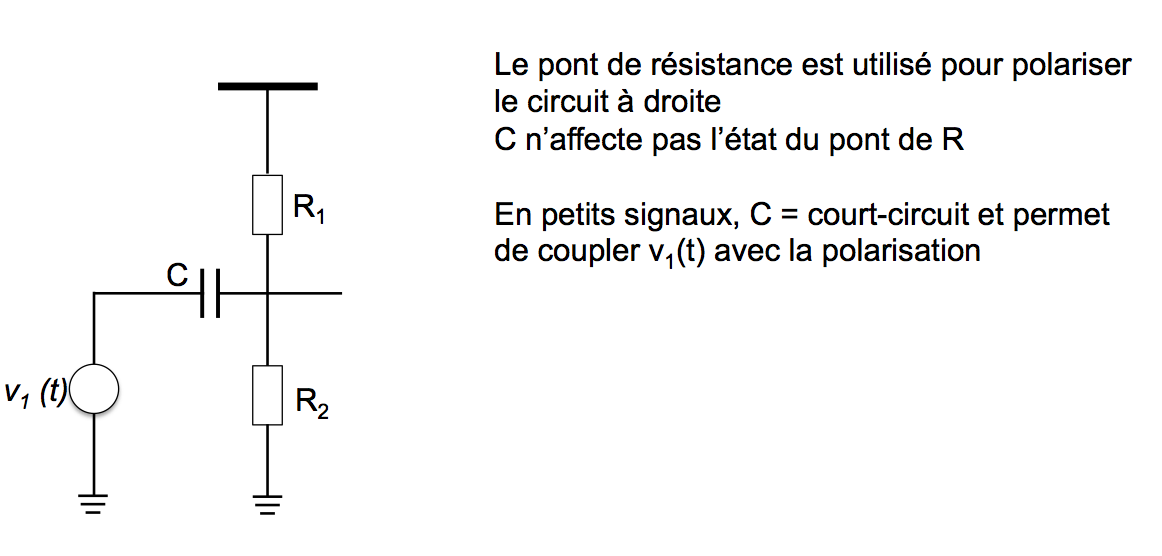
\includegraphics[scale=0.5]{couplage}
\subsubsection{Condensateurs de détournement}
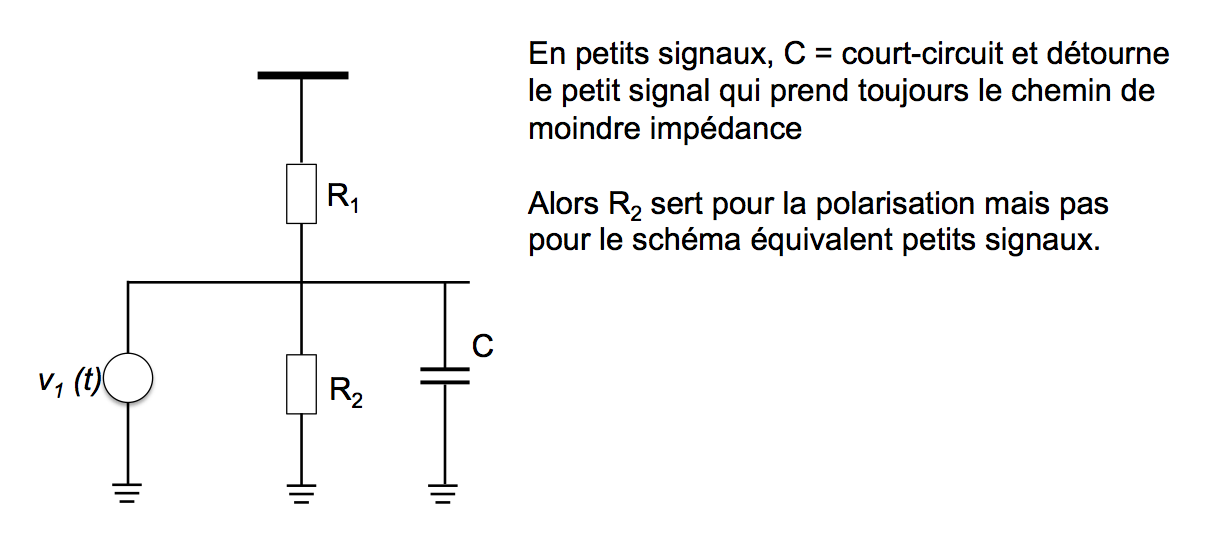
\includegraphics[scale=0.5]{det}

\subsection{Objectif}
Fixer le point de fonctionnement P (aussi appelé \textbf{point de Polarisation}) du transistor de façon indépendante de la dispersion caractéristique des transistors, en assurant sa stabilité, notamment vis-à-vis de la température, et en limitant le nombre de sources d'alimentation. C'est autour de ce point que prendront place les variations à amplifier.

\subsubsection{Variations et imperfections}
\begin{itemize}
\item \textbf{Variation de température :}

\begin{itemize}
\item $I_C = cst \Rightarrow V_{BE}$ varie de $ -2mV/K$ 
\item  $V_{BE} = cst \Rightarrow I_{C}$ augmente de $ 8\%/K$ 
\item $\beta$ augmente de $ 0.8-1.5\%/K$  
 
\end{itemize}


\item \textbf{Dispersion des paramètres du transistor (tolérances) :}

\begin{itemize}
\item \textbf{$I_S$ :} $\pm 50\%$
\item \textbf{$\beta$ :} $\pm 100\%$
\end{itemize}

\end{itemize}

\subsubsection{Polarisation par base}
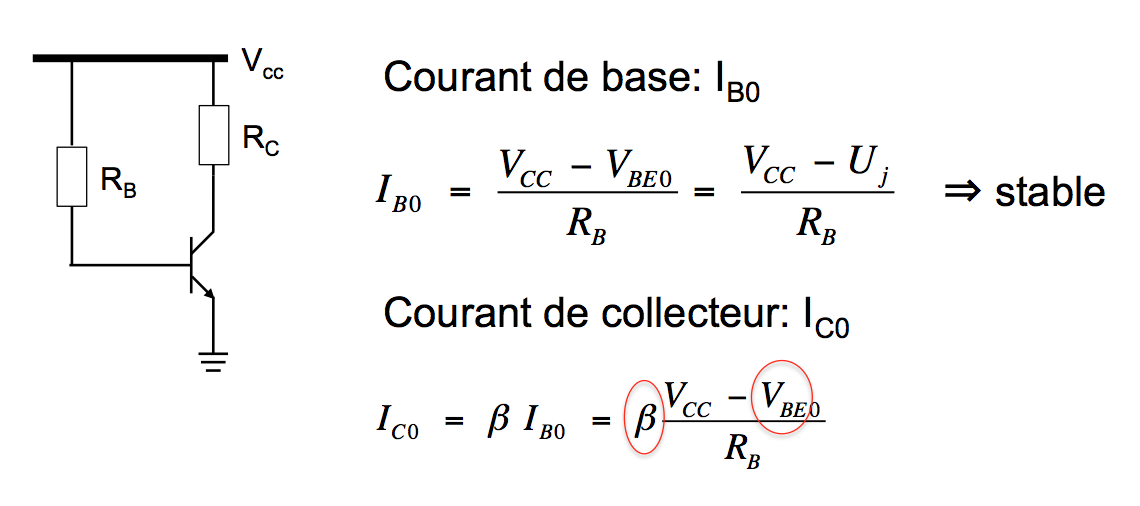
\includegraphics[scale=0.5]{polbase}
\subsubsection{Polarisation par l'émetteur}
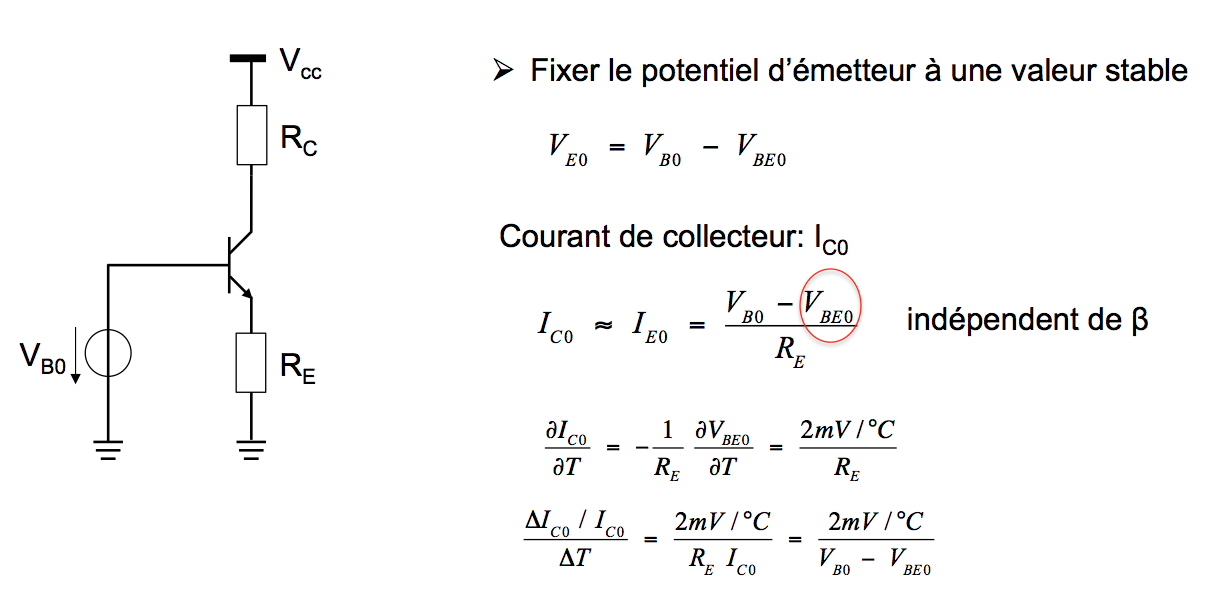
\includegraphics[scale=0.5]{polem}
\subsubsection{Polarisation par contrôle du courant d'émetteur}
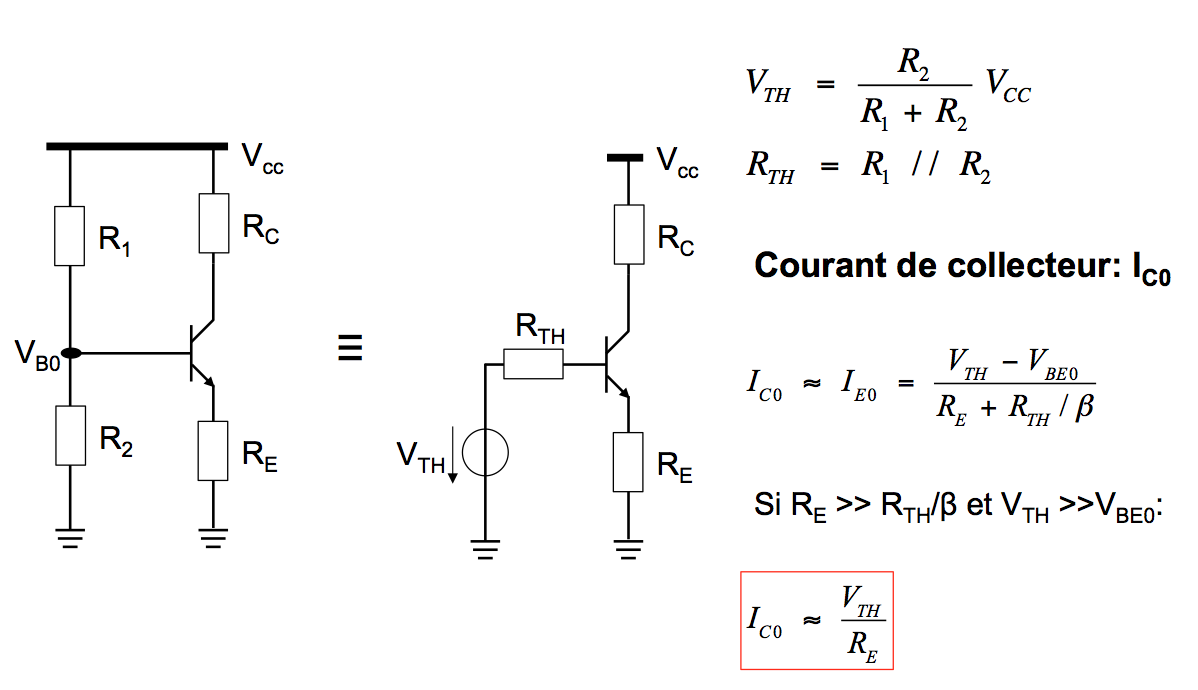
\includegraphics[scale=0.3]{polcourem}
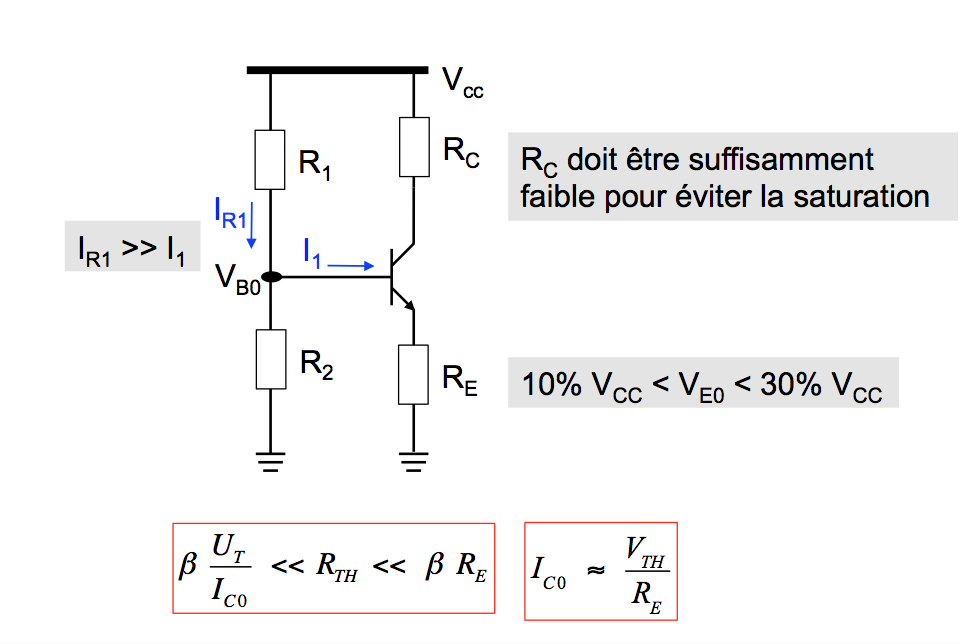
\includegraphics[scale=0.3]{polcourem2}

\subsubsection{Polarisation par contre-réaction collecteur-base}
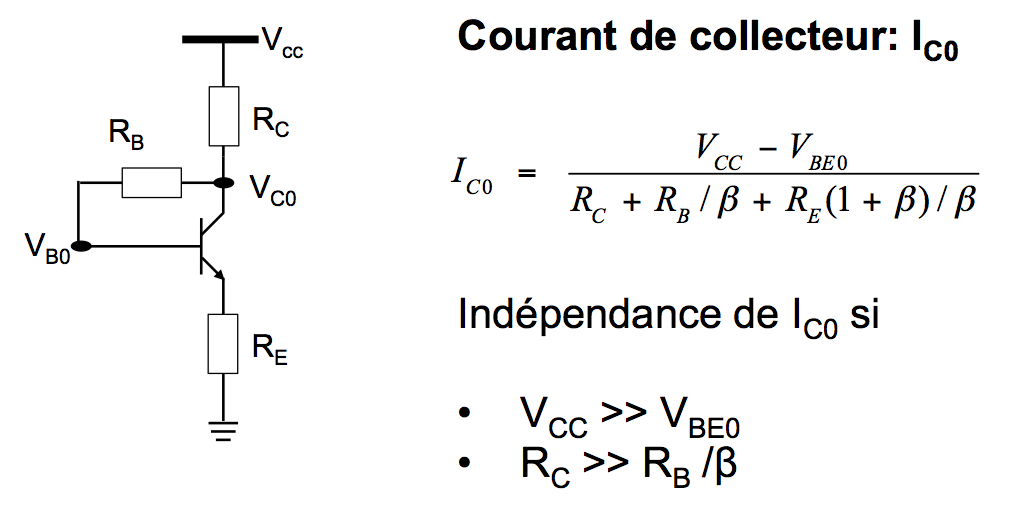
\includegraphics[scale=0.5]{polcolbase}

\section{Sources de courant}
\subsection{Montage de Base}
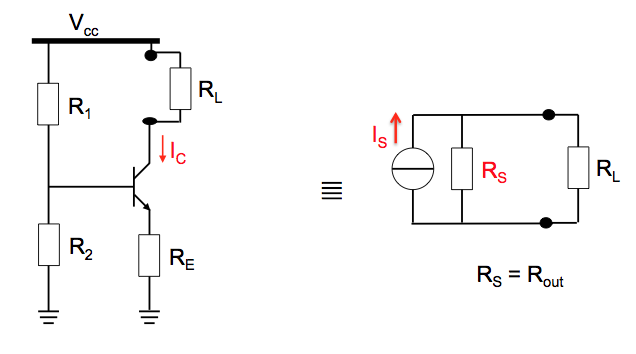
\includegraphics[scale=0.7]{courant}

En mode normal, $I_C$ est quasi-indépendant de $V_{CE}$. On notera aussi que $R_{source}$ est très élevée.
On a : $$ I_C = \frac{V_{TH} - V_{BE}}{R_E + \frac{R_{TH}}{\beta}} = I_{source}$$
$$ V_{CE} > 0 \Rightarrow R_L < \frac{V_{CC}}{I_L} - V_E $$
$$ R_{out} = \frac{1}{g_{ce}}(1+\frac{\beta R_E}{R_E+ R_{TH}+ \frac{1}{g_{BE}}})+(R_{TH}+\frac{1}{g_{be}})//R_E$$
\textbf{NB :} Si $R_E = 0 \Rightarrow R_{out} = \frac{1}{g_{ce}}$

\subsection{Miroir de courant}





\end{document}